\documentclass{article}

\renewcommand{\familydefault}{\sfdefault}  %serifenlose Schrift
\usepackage{helvet} % Schrift: Helvetica


\usepackage{graphicx,graphics,tikz}
\usepackage{amsmath}
\usepackage{amsthm}
\usepackage{amsfonts}
\usepackage{amssymb}
\usepackage{marvosym} % to be able to show male and female symbols with: \Female and \Male
\usepackage{gensymb}
\usepackage[graphics,tightpage,active]{preview}
\PreviewEnvironment{tikzpicture}
\newlength\imagewidth
\newlength\imagescale

\begin{document}

\pgfmathsetlength{\imagewidth}{10cm} % desired displayed width of image
\pgfmathsetlength{\imagescale}{\imagewidth/2000} % pixel width of image
% adjust scale of tikzpicture (and direction of y) such that pixel
% coordinates can be used for drawing overlays:
\usetikzlibrary{backgrounds}

\begin{tikzpicture}[x=\imagescale,y=-\imagescale]

  % Insert Background Image place image (integer coordinates refer to

\node at (0cm, 0cm) {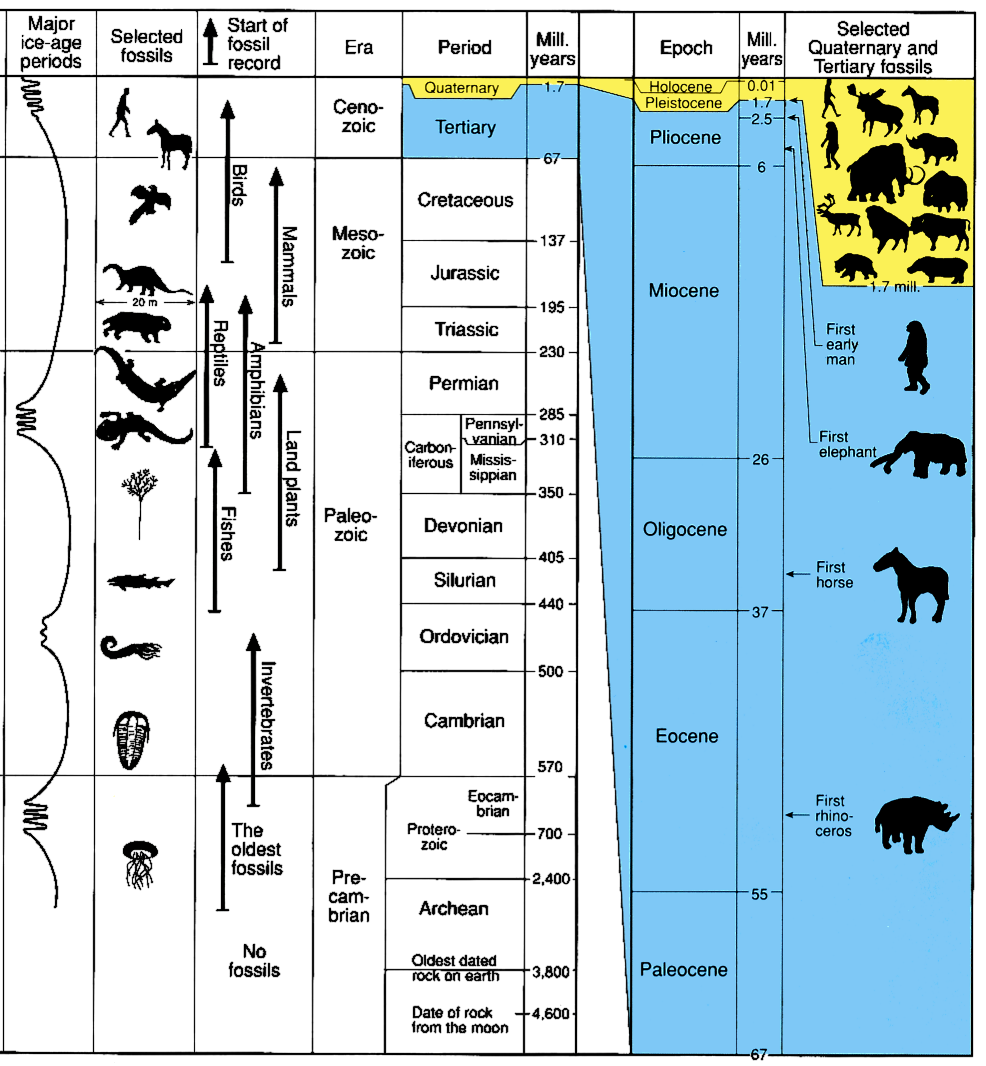
\includegraphics[height=7.3cm]{Andersen-1997-Fig1-31.png}};
\node (iceages) [anchor=east] at (-5cm,1.5cm) {\alert{\small{Ice age periods}}};
\node (a) at (-3.2cm,3cm) {};
\node (b) at (-3.2cm,0.8cm) {};
\node (c) at (-3.1cm,-0.7cm) {};
\node (d) at (-3.2cm,-1.9cm) {};
\draw [color=red,-latex,line width=0.02cm] (iceages) to [out=0,in=180] (a);
\draw [color=red,-latex,line width=0.02cm] (iceages) to [out=0,in=180] (b);
\draw [color=red,-latex,line width=0.02cm] (iceages) to [out=0,in=180] (c);
\draw [color=red,-latex,line width=0.02cm] (iceages) to [out=0,in=180] (d);

\draw  [color=red,line width=0.02cm] (-3.2cm,3cm) circle (0.3cm);


\node (25)  [color=red,anchor=east] at (-5cm,2.9cm) {\small{2.5 Mya}};
\node (45) [color=red,anchor=east] at (-5cm,-3.3cm) {\small{4,6 Bya}};

\node (252) at (-3.5cm,2.9cm) {};
\node (452) at (-3.5cm,-3.3cm) {};

\draw [color=red,line width=0.02cm] (25) to [out=0,in=180] (252);
\draw [color=red,line width=0.02cm] (45) to [out=0,in=180] (452);

\end{tikzpicture}

\end{document}